\documentclass[11pt]{article}
\usepackage{fontspec}
\setmainfont{NotoSerif-Regular.ttf}[Path=C:/Windows/Fonts/,ItalicFont=NotoSerif-Italic.ttf,BoldFont=NotoSerif-Bold.ttf,BoldItalicFont=NotoSerif-BoldItalic.ttf]
\usepackage[a4paper,margin=22mm]{geometry}
\usepackage{amsmath,amssymb,graphicx,xcolor,hyperref,needspace,tikz}
\usepackage[normalem]{ulem}
\let\MathUnderline\underline
\renewcommand{\underline}[1]{\ifmmode\MathUnderline{#1}\else\uline{#1}\fi}
\hypersetup{unicode=true,colorlinks=true,linkcolor=blue,pdfauthor={}}
\setlength{\parindent}{0pt}
\setlength{\parskip}{.4em}
\setlength{\emergencystretch}{3em}
\raggedright
\newcommand{\SourcePage}[2]{\par\smallskip\phantomsection\label{#1:source-page}{\small\sffamily\color{blue!55!black}#1}\par\smallskip}
\newcommand{\EvidenceBlock}[4]{%
 \par\smallskip\noindent\begin{minipage}{\linewidth}
 \begin{minipage}[t]{.47\linewidth}\vspace{0pt}\centering
 \csname evidence-#1-#2\endcsname\par
 {\scriptsize\SourceCropCaption\ #1}\par
 \end{minipage}\hfill
 \begin{minipage}[t]{.49\linewidth}\vspace{0pt}\raggedright
 {\small\color{orange!65!black}\textbf{#4} #3}\par
 \end{minipage}
 \end{minipage}\par\smallskip}
\newcommand{\Unclear}[3]{\EvidenceBlock{#1}{#2}{#3}{\ReadingCaption}}
\newcommand{\Incomplete}[3]{\EvidenceBlock{#1}{#2}{#3}{\IncompleteCaption}}
\newcommand{\SourceFigure}[3]{\EvidenceBlock{#1}{#2}{#3}{\DiagramCaption}}
\expandafter\def\csname evidence-GELFAND-P000001-module-letter\endcsname{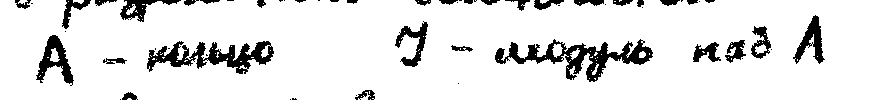
\includegraphics[width=\linewidth]{figures/gelfand-p000001-module-letter-original.png}}
\expandafter\def\csname evidence-GELFAND-P000001-diagram-blowup\endcsname{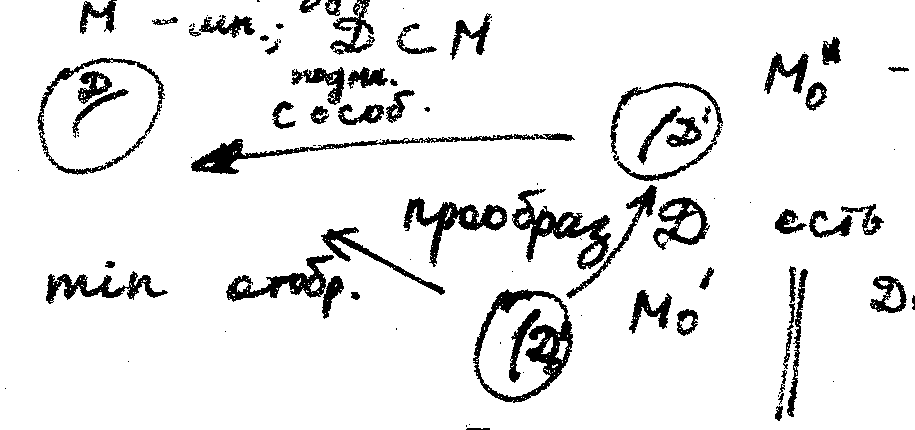
\includegraphics[width=\linewidth]{figures/gelfand-p000001-diagram-blowup-original.png}}
\expandafter\def\csname evidence-GELFAND-P000001-blowup-notation\endcsname{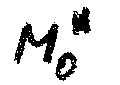
\includegraphics[width=.43\linewidth]{figures/gelfand-p000001-upper-blowup-label-original.png}\hfill
\includegraphics[width=.50\linewidth]{figures/gelfand-p000001-lower-blowup-label-original.png}}
\expandafter\def\csname evidence-GELFAND-P000001-origin-example\endcsname{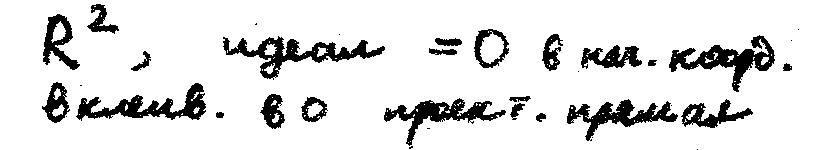
\includegraphics[width=\linewidth]{figures/gelfand-p000001-origin-example-original.png}}
\newcommand{\SourceCropCaption}{Original source details:}\newcommand{\ReadingCaption}{Uncertain reading.}\newcommand{\IncompleteCaption}{Undeciphered passage.}\newcommand{\DiagramCaption}{Diagram and typed description.}
\hypersetup{pdftitle={Gelfand seminar — chapter 1}}

\expandafter\def\csname evidence-GELFAND-P000002-ideal-selection\endcsname{
\includegraphics[width=\linewidth]{figures/gelfand-p000002-ideal-selection-part01-original-r1.png}}
\expandafter\def\csname evidence-GELFAND-P000002-open-set-notation\endcsname{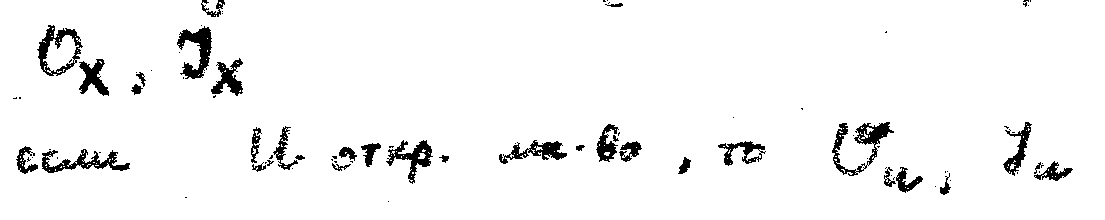
\includegraphics[width=\linewidth]{figures/gelfand-p000002-open-set-notation-part01-original-r2.png}}
\expandafter\def\csname evidence-GELFAND-P000002-fractions-sentence\endcsname{
\includegraphics[width=\linewidth]{figures/gelfand-p000002-fractions-sentence-part01-original-r1.png}\par\smallskip
\includegraphics[width=\linewidth]{figures/gelfand-p000002-fractions-sentence-part02-original-r1.png}\par\smallskip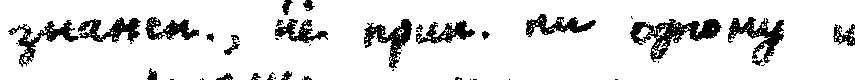
\includegraphics[width=\linewidth]{figures/gelfand-p000002-fractions-sentence-part03-original-r1.png}\par\smallskip
\includegraphics[width=\linewidth]{figures/gelfand-p000002-fractions-sentence-part04-original-r1.png}}
\expandafter\def\csname evidence-GELFAND-P000002-margin-grothendieck\endcsname{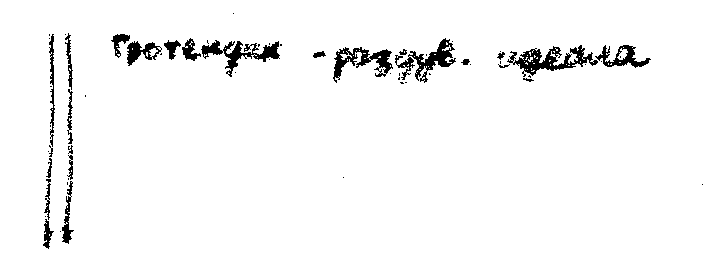
\includegraphics[width=\linewidth]{figures/gelfand-p000002-margin-grothendieck-part01-original-r1.png}}
\expandafter\def\csname evidence-GELFAND-P000002-quadratic-coefficients\endcsname{
\includegraphics[width=\linewidth]{figures/gelfand-p000002-quadratic-coefficients-part01-original-r1.png}}
\expandafter\def\csname evidence-GELFAND-P000002-last-sign\endcsname{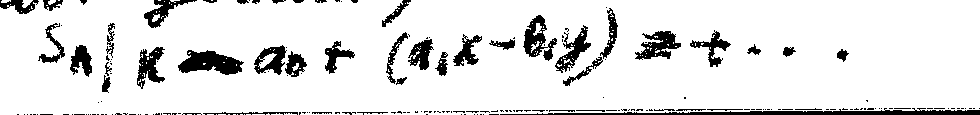
\includegraphics[width=\linewidth]{figures/gelfand-p000002-last-sign-part01-original-r1.png}}
\expandafter\def\csname evidence-GELFAND-P000003-directions\endcsname{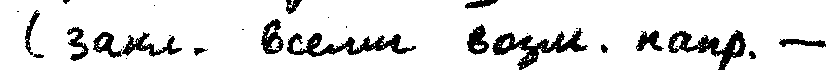
\includegraphics[width=\linewidth]{figures/gelfand-p000003-directions-part01-original-r1.png}\par\smallskip
\includegraphics[width=\linewidth]{figures/gelfand-p000003-directions-part02-original-r1.png}}
\expandafter\def\csname evidence-GELFAND-P000003-cross-cancellation\endcsname{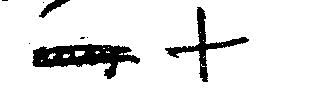
\includegraphics[width=\linewidth]{figures/gelfand-p000003-cross-cancellation-part01-original-r1.png}}
\expandafter\def\csname evidence-GELFAND-P000003-ising-cancellation\endcsname{
\includegraphics[width=\linewidth]{figures/gelfand-p000003-ising-cancellation-part01-original-r1.png}}
\expandafter\def\csname evidence-GELFAND-P000003-configuration-letter\endcsname{
\includegraphics[width=\linewidth]{figures/gelfand-p000003-configuration-letter-part01-original-r2.png}}
\expandafter\def\csname evidence-GELFAND-P000003-energy-cancellation\endcsname{
\includegraphics[width=\linewidth]{figures/gelfand-p000003-energy-cancellation-part01-original-r1.png}}
\expandafter\def\csname evidence-GELFAND-P000003-energy-case\endcsname{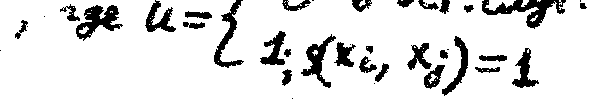
\includegraphics[width=\linewidth]{figures/gelfand-p000003-energy-case-part01-original-r2.png}\par\smallskip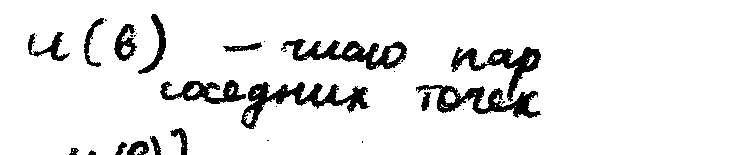
\includegraphics[width=\linewidth]{figures/gelfand-p000003-energy-case-part02-original-r3.png}}
\expandafter\def\csname evidence-GELFAND-P000003-partition-domain\endcsname{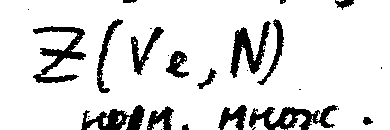
\includegraphics[width=\linewidth]{figures/gelfand-p000003-partition-domain-part01-original-r1.png}\par\smallskip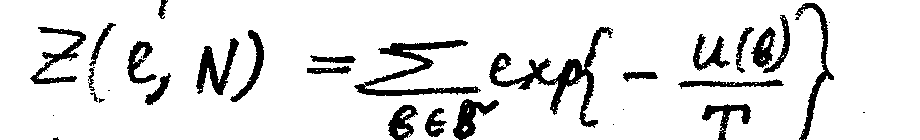
\includegraphics[width=\linewidth]{figures/gelfand-p000003-partition-domain-part02-original-r1.png}}
\expandafter\def\csname evidence-GELFAND-P000003-attraction-note\endcsname{
\includegraphics[width=\linewidth]{figures/gelfand-p000003-attraction-note-part01-original-r1.png}}
\expandafter\def\csname evidence-GELFAND-P000003-density-cancellation\endcsname{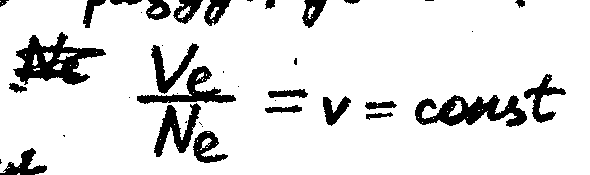
\includegraphics[width=\linewidth]{figures/gelfand-p000003-density-cancellation-part01-original-r1.png}}
\begin{document}
{\large\bfseries Gelfand seminar — chapter 1}\par
{\small Opening of the reader. Source frames 1–3. Text and formulas are typed; original details accompany every uncertain reading. Working excerpt; the complete chapter is still in preparation.}\par\medskip
\SourcePage{GELFAND-P000001}{unlabelled}
Monday, $21/\mathrm{IX}$.
Cartesian and Boolean products of groups.

``Hironaka: on resolution of singularities.''
\underline{Gelfand}

$A$ is a ring, $\mathcal{J}$ is a module over $A$.
\Unclear{GELFAND-P000001}{module-letter}{The letter for the module and ideal is rendered as $\mathcal{J}$; $\mathcal{I}$ or $J$ are possible.}

Blow-up --- ?
$M$ is a manifold; $D\subset M$.
[Beneath $D$:] a subset with singularities.

$M_0^H$ is the blow-up. Blowing-up.
The inverse image of $D$ is $D'$, a manifold of dimension $n-1$.
$D_0$ is $(n-1)$-dimensional.
\SourceFigure{GELFAND-P000001}{diagram-blowup}{Three enclosed drawings: at left a region with $D$; at upper right a region with $D'$ and the label $M_0^H$; at lower right a region and the label $M'_0$. The upper arrow points left; the lower oblique arrow also points left, with the label ``continuous map'' [source abbreviation: непр. отобр.]. The precise inner curves, labels and the connection of the lower region to the upper one require comparison with the scan.}
\Unclear{GELFAND-P000001}{blowup-notation}{The upper index on $M_0$ resembles $H$; the lower region's label resembles $M'_0$.}

The construction is Grothendieck's.
$A$ is a ring, $\mathcal{J}$ is a module.
\underline{Example.} $A$ is a ring of functions;
$\mathcal{J}$ is the ideal of functions taking the value $0$ on $D$.

One obtains a sheaf of rings and a sheaf of modules.
$A$ is a ring, $\mathcal{J}$ is an ideal.
Construct $X$, $O_X$ a sheaf of rings,
$\mathcal{J}_X$ a sheaf of ideals, so that
\begin{gather*}
 (A,\mathcal{J})\ \longleftarrow\ (X,O_X,\mathcal{J}_X).
\end{gather*}
[Beneath the arrow:] linear map.

$(A,\mathcal{J})$ is a sheaf generated by $1$ ideal.

$\mathcal{J}_X$ is invertible, i.e. an ideal of the ring:
$\exists f\in\mathcal{J}_X$ such that $O_Xf=\mathcal{J}_X$.
[Above the formula, an arrow to $\exists$:] generator.

(The ideal is principal if $\mathcal{J}$ is an ideal.)
Then the zero variety is $1$ equation.

$A$ is a ring, $\mathcal{J}$ is an ideal.
\underline{Typical example:} $R^2$, the ideal $=0$ at the origin.
\Unclear{GELFAND-P000001}{origin-example}{The next line: ``Gluing a projective line into $0$'' [source: Вклеив. в $0$ проект. прямой]; the beginning may read ``Оклеив.''.}

$A$, $\mathcal{J}$ are modules.
\begin{gather*}
 \mathcal{J}\otimes_A\mathcal{J},\qquad
 \mathcal{J}\otimes_A\mathcal{J}\otimes_A\mathcal{J},\ldots
\end{gather*}
[Above the groups of tensor products:] symmetric; symmetric.

Consider formal sums
\begin{gather*}
 \sum_{k=0}^{N}a_kz^k.
\end{gather*}
Add and multiply.
$x\otimes y=y\otimes x$.
\begin{gather*}
 a_0\in A,\qquad a_1\in\mathcal{J},\qquad
 a_2\in\mathcal{J}\otimes_A\mathcal{J}\quad\text{—}
\end{gather*}

\SourcePage{GELFAND-P000002}{unlabelled}
The ring of these sums is $S_A(\mathcal{J})$.
Consider homogeneous ideals
[inserted above the line:] (graded).
(Together with a polynomial it contains all its homogeneous components.)

Consider all homogeneous prime ideals in $S_A(\mathcal{J})$.
Выбр. [source abbreviation] ideals which contain all polynomials, starting with degree $1$.
\Unclear{GELFAND-P000002}{ideal-selection}{The end of the line after ``contain all'' is better read as ``polynomials, starting with degree $1$''; the middle strokes of the abbreviation ``нач.'' remain indistinct.}

The collection of ideals is $X$. (The Zariski topology.)
$O_X$, $\mathcal{J}_X$.
If $U$ is an open set, then $O_U$, $\mathcal{J}_U$.
\Unclear{GELFAND-P000002}{open-set-notation}{After ``then'', the first letter has the same form as $O_X$ above, the second as the ideal letter: $O_U$, $\mathcal{J}_U$; the latter may be $\mathcal{I}_U$.}

$S_A(\mathcal{J})$ is the whole ring.
The ring of fractions, numerators, denominators, not belonging to any of the ideals.
Localize the ring at this set.
Fractions of degree $1$: $\mathcal{J}_U$.
\Unclear{GELFAND-P000002}{fractions-sentence}{In the line about fractions, the abbreviations ``numerator--denominator'' and whether ``not belonging'' applies only to the denominator are unclear. No words are supplied from the meaning.}
[At right, two downward arrows:] Grothendieck --- blow up ideally.
\Unclear{GELFAND-P000002}{margin-grothendieck}{The right-hand note reads ``Grothendieck --- blow up ideally''; the last word may be ``идеально'' [ideally] or ``идеалы'' [ideals].}

$A$ is the ring of polynomials in $2$ variables.
$\mathcal{J}$ is the ideal of polynomials with $P(0,0)=0$.
\begin{gather*}
 A=\{P(x,y)\},\qquad
 \mathcal{J}=P(x,y)=a_1x+b_1y+\cdots .
\end{gather*}
\begin{gather*}
 \mathcal{J}\otimes_A\mathcal{J}\ \longleftrightarrow
 \{a_2x^2+2b_2xy+cy^2+\cdots\}.
\end{gather*}
\Unclear{GELFAND-P000002}{quadratic-coefficients}{The coefficients in the quadratic polynomial read $a_2$, $2b_2$, $c$; the index on $c$ and the shape of the thick two-headed arrow are uncertain.}

Because of the interchange, one obtains the same as the square of the ideal.
Then --- the ideal of polynomials equal to $0$ at this point.
What will it blow up into? ?

\begin{gather*}
 \sum P_k(x,y)z^k,\qquad P_k(x,y)=ax^k+\cdots .
\end{gather*}
[At right:] Graded $\Sigma$ of tensor products.
\begin{gather*}
 A=\{P_0(x,y)\}\longrightarrow S_A(\mathcal{J}),\qquad
 P_0(x,y)\sim P_0(x,y).
\end{gather*}
The set of prime ideals obtained from the ideal $P(0,0)=0$.
\begin{gather*}
 S_A\sim\sum P_kz^k,\qquad P_k\in\mathcal{J}^k,\qquad
 K\sim\sum P_kz^k.
\end{gather*}
It suffices to find the max. ideals of the quotient ring ---
(to find the ideals containing the given one).
\begin{gather*}
 S_A/K\ \longleftrightarrow\ a_0+(a_1x-b_1y)z+\cdots .
\end{gather*}
\Unclear{GELFAND-P000002}{last-sign}{In the last formula a minus is visible before $b_1y$, although the next scan has a plus. The visible minus is retained; the direction of the thick arrow is also uncertain.}

\SourcePage{GELFAND-P000003}{2}
All homogeneous max. ideals in it will be the points of the extension.
There is no constant term (then also $1$).
\begin{gather*}
 (a_1x+b_1y)z.
\end{gather*}
Only $1$ linear combination of $x$ and $y$.
(Not $2$, since then all.)

The ideals determine directions in the plane
(замк. [source abbreviation] with all possible directions --- the $\sigma$-process).
\Unclear{GELFAND-P000003}{directions}{The abbreviations in parentheses read ``замк. всеми возм. напр.''; neither the first word nor the meaning of the sign $\sigma$ is asserted.}
\Needspace{48mm}\underline{Problem.} In the space
[cancelled:] \Unclear{GELFAND-P000003}{cross-cancellation}{The cancelled word before the drawing is illegible.}
\par\smallskip\noindent\begin{minipage}{\linewidth}\begin{minipage}[t]{.47\linewidth}\centering\vspace{0pt}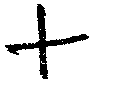
\includegraphics[width=30mm]{figures/gelfand-p000003-cross-diagram-original-r1.png}\par{\scriptsize Original diagram}\end{minipage}\hfill\begin{minipage}[t]{.49\linewidth}\centering\vspace{0pt}\begin{tikzpicture}[scale=0.5]
 \draw (-0.8,0)--(0.8,0);
 \draw (0,-0.7)--(0,0.8);
\end{tikzpicture}\par{\scriptsize Typeset recreation}\end{minipage}\end{minipage}\par\smallskip
What results from gluing it in?
\begin{gather*}
 z=0,\qquad xy=0,\qquad \mathcal{J}=(z,xy).
\end{gather*}
[A line is drawn beneath the system.]

\underline{Dobrushin.}
[Cancelled before ``Find'':] \Unclear{GELFAND-P000003}{ising-cancellation}{The cancelled beginning of the line cannot be read confidently.}
Find an example of a gas in which phase transitions occur.
A cube of the integer lattice.
$\ell$ is the length. $V_\ell=\ell^\nu$.
$N$ points, $N<V_\ell$.
They can occupy positions on the lattice
$\theta=(x_1,\ldots,x_N)$.
\Unclear{GELFAND-P000003}{configuration-letter}{The configuration sign is rendered as $\theta$; the handwritten sign also resembles $b$ or Cyrillic ``в''.}

The Ising model.
[Before the formula, a densely cancelled sign:]
\Unclear{GELFAND-P000003}{energy-cancellation}{The separate cancelled sign before $U(\theta)$ is illegible.}
\begin{gather*}
 U(\theta)=-\frac12\sum_{i\ne j}u(x_i,x_j),\qquad
 u=\begin{cases}
 0&\text{in the other cases},\\
 1;&\rho(x_i,x_j)=1.
 \end{cases}
\end{gather*}
$u(\theta)$ is the number of pairs of neighboring points.
\Unclear{GELFAND-P000003}{energy-case}{In the condition for the second branch a sign resembling $\rho$ is visible; the semicolon after $1$ is retained. In the caption below, the first letter resembles lowercase $u$ rather than $U$.}

The basic axiom is the Gibbs distribution.
\begin{gather*}
 \mathsf{P}(B)=
 \frac{\displaystyle\sum_{\theta\in B}\exp\{-U(\theta)/T\}}
 {Z(V_\ell,N)},\qquad T>0\text{ --- temperature.}
\end{gather*}
[Beneath the denominator:] normalizing factor.
\begin{gather*}
 Z(\ell,N)=\sum_{\theta\in\mathcal{B}}\exp\{-U(\theta)/T\}.
\end{gather*}
\Unclear{GELFAND-P000003}{partition-domain}{The denominator in the first formula reads $Z(V_\ell,N)$, the next line $Z(\ell,N)$; the set sign beneath the sum resembles $\mathcal{B}$. The notation is not adjusted for consistency.}

The molecules attract one another.
([Two filled signs with arrows:] neighbors $>$ their probability.)
\Unclear{GELFAND-P000003}{attraction-note}{In parentheses after ``The molecules attract'', there are filled signs and arrows; the reading ``neighbors $>$ their probability'' is uncertain.}
$B\subset\mathcal{B}$ is a collection of configurations.
\begin{gather*}
 p(\theta)=\frac{\exp\{-U(\theta)/T\}}{Z(\ell,N)}.
\end{gather*}
Take the limit $\ell\to\infty$; the cube expands to $\infty$.
$N_\ell$ depends on $\ell$.
[A cancelled sign before the fraction:]
\Unclear{GELFAND-P000003}{density-cancellation}{The cancelled sign before $V_\ell/N_\ell$ is illegible.}
\begin{gather*}
 \frac{V_\ell}{N_\ell}=v=\mathrm{const}.
\end{gather*}
The lattice grows.
One can show that
\begin{gather*}
 \frac1{N_\ell}\log Z(\ell,N_\ell)\longrightarrow f(v,T).
\end{gather*}
\clearpage\section*{Full reading notes}
\subsection*{GELFAND-0001-U001}
\EvidenceBlock{GELFAND-P000001}{module-letter}{After “A is a ring” is a handwritten letter with a fork at the top and a lower hook; it recurs for the module and the ideal.}{Observation.}
\par\smallskip\noindent\textbf{Candidates: } \(\mathcal{J}\); \(\mathcal{I}\); J\par
\par\smallskip\noindent\textbf{Historical note: } A calligraphic J was used in the text as a graphical candidate; the notation was not identified from its mathematical meaning.\par
\par\smallskip\noindent\textbf{Fresh source comparison: } The same fork and lower hook are visible in three separate occurrences at 5×/10×. This supports a consistent graphical transcription but does not distinguish every possible conventional I/J letterform.\par
\subsection*{GELFAND-0001-U002}
\EvidenceBlock{GELFAND-P000001}{diagram-blowup}{In the upper half are three rounded contours with inner curves and two leftward arrows; D, D-prime, M and indices occur above and beside them.}{Observation.}
\par\smallskip\noindent\textbf{Candidates: } None proposed.\par
\par\smallskip\noindent\textbf{Historical note: } Uncertain inner curves and joins were not redrawn. The description and the source-figure entry retain a locator for comparison.\par
\par\smallskip\noindent\textbf{Fresh source comparison: } The complete diagram crop is now displayed at its typed description. Both leftward arrowheads are visible. A separate curved stroke rises from the lower contour toward the area beside D; its exact attachment to the upper contour is not asserted.\par
\subsection*{GELFAND-0001-U003}
\EvidenceBlock{GELFAND-P000001}{blowup-notation}{The upper index on \(M_0\) resembles H; over \(M_0\) at the lower region is a short stroke.}{Observation.}
\par\smallskip\noindent\textbf{Candidates: } \(M_0^H\); \(M'_0\); \(M_0^N\); \(M'_0\)\par
\par\smallskip\noindent\textbf{Historical note: } The indices and prime need comparison with the original.\par
\par\smallskip\noindent\textbf{Fresh source comparison: } Separate close crops show the dark upper index and the lower prime at the reading itself. The lower prime is distinct; the dark upper sign still does not justify excluding N in favor of H.\par
\subsection*{GELFAND-0001-U006}
\EvidenceBlock{GELFAND-P000001}{origin-example}{To the right of the \(R^2\) example the line begins with a joined group of letters and ends “into 0, a projective line”.}{Observation.}
\par\smallskip\noindent\textbf{Candidates: } Вклеив. в 0 проект. прямой [Gluing a projective line into 0]; Оклеив. в 0 проект. прямой [alternative initial abbreviation]\par
\par\smallskip\noindent\textbf{Historical note: } The phrase is given inside the uncertain-reading entry, without choosing from the mathematical meaning of a blow-up.\par
\par\smallskip\noindent\textbf{Fresh source comparison: } The wider context and 5×/10× details strongly favor the initial В and the abbreviation Вклеив. The historical alternative remains visible; the source wording is not replaced by a standard construction of a blow-up.\par

\subsection*{GELFAND-0001-U007}
\EvidenceBlock{GELFAND-P000002}{ideal-selection}{A rereading of the enlarged original fragment favors “polynomials, starting with degree 1”; the middle strokes of the abbreviation нач. are still not fully distinguishable.}{Observation.}
\par\smallskip\noindent\textbf{Candidates: } мн., нач. с 1-й степени [polynomials, starting with degree 1]; мн., к-ст. с 1-й степенью [alternative abbreviation; expansion uncertain]\par
\par\smallskip\noindent\textbf{Historical note: } The first candidate was selected from the shape of the original line; it was not replaced by the standard definition of Proj.\par
\par\smallskip\noindent\textbf{Fresh source comparison: } The line ending is visible in the wider crop and separate 5×/10× details. Its first abbreviation Выбр. is visible too, but its expansion could express selecting or discarding. The English text retains that abbreviation rather than deciding the operation from the construction. The strokes favor нач. at the end; the historical alternative remains recorded.\par

\subsection*{GELFAND-0001-U008}
\EvidenceBlock{GELFAND-P000002}{open-set-notation}{In a separate rereading, the first letter after “then” matches the shape of \(O_X\) above; the second matches the ideal letter with a lower hook.}{Observation.}
\par\smallskip\noindent\textbf{Candidates: } \(O_U,J_U\); \(O_U,I_U\)\par
\par\smallskip\noindent\textbf{Historical note: } The initial reading of the first letter as J was corrected from the scan. The possible I/J distinction in the second letter remains, independently of the standard sheaf construction.\par
\par\smallskip\noindent\textbf{Fresh source comparison: } The corrected context now includes the whole lower subscripts. The rounded first sign and forked, hooked second sign match the earlier pair. These shapes support O followed by the ideal letter, without deciding every conventional I/J distinction. Separate 5×/10× details were inspected.\par

\subsection*{GELFAND-0001-U009}
\EvidenceBlock{GELFAND-P000002}{fractions-sentence}{After “ring of fractions” one can see “numer., denom., not belonging to any of the ideals”, but the abbreviation boundaries and the scope of the last phrase are unclear.}{Observation.}
\par\smallskip\noindent\textbf{Candidates: } числ., знамен., не прин. ни одному из идеалов [numer., denom., not belonging to any of the ideals]; числ.; знамен. не прин. ни одному из идеалов [numer.; denom. not belonging to any of the ideals]\par
\par\smallskip\noindent\textbf{Historical note: } The punctuation was not corrected from the definition of localization.\par
\par\smallskip\noindent\textbf{Fresh source comparison: } Four overlapping source parts retain the line ending числ., the following знамен., and the phrase about the ideals. The abbreviations are visible at 5×/10×; their punctuation does not establish which nouns the restriction modifies. No missing qualifier is supplied.\par

\subsection*{GELFAND-0001-U010}
\EvidenceBlock{GELFAND-P000002}{margin-grothendieck}{The right-hand note beside two vertical arrows reads “Grothendieck — blow up …”; the final word is written continuously.}{Observation.}
\par\smallskip\noindent\textbf{Candidates: } идеально [ideally]; идеалы [ideals]\par
\par\smallskip\noindent\textbf{Historical note: } The final word is not asserted.\par
\par\smallskip\noindent\textbf{Fresh source comparison: } The wider crop includes both downward arrows and the full note. The joined final strokes favor идеально, but do not securely exclude идеалы. The literal candidate “blow up ideally” is retained with the alternative; the wording is not regularized into a definition.\par

\subsection*{GELFAND-0001-U011}
\EvidenceBlock{GELFAND-P000002}{quadratic-coefficients}{After J tensor J is a thick two-sided mark and a quadratic polynomial; the coefficients resemble \(a_2\), \(2b_2\), c.}{Observation.}
\par\smallskip\noindent\textbf{Candidates: } \(a_2x^2+2b_2xy+cy^2+\cdots\); \(a_2x^2+2b_2xy+c_2y^2+\cdots\)\par
\par\smallskip\noindent\textbf{Historical note: } The index on the final coefficient and the direction of the thick mark are uncertain.\par
\par\smallskip\noindent\textbf{Fresh source comparison: } The complete context and separate details show \(a_2\) and \(2b_2\). A small upper stroke is visible near the c-shaped coefficient; it is not a secure lower index 2. The thick connecting mark is retained as an uncertain graphical candidate, without inferring an isomorphism.\par

\subsection*{GELFAND-0001-U012}
\EvidenceBlock{GELFAND-P000002}{last-sign}{At the lower edge is \(a_0+(a_1x-b_1y)z+\cdots\); the horizontal sign before \(b_1y\) looks like a minus.}{Observation.}
\par\smallskip\noindent\textbf{Candidates: } \(a_0+(a_1x-b_1y)z+\cdots\); \(a_0+(a_1x+b_1y)z+\cdots\)\par
\par\smallskip\noindent\textbf{Historical note: } The visible minus is retained in the body; the next scan has a plus. The arrow at left is written heavily.\par
\par\smallskip\noindent\textbf{Fresh source comparison: } The enlarged sign is a horizontal minus; no vertical crossing stroke is visible. The next source page has a plus. Both source readings remain, and the mathematical commentary does not use a change of sign to alter either transcription. The heavy arrow still has uncertain direction.\par

\subsection*{GELFAND-0001-U013}
\EvidenceBlock{GELFAND-P000003}{directions}{In parentheses after “plane” is the abbreviation “замк. всеми возм. напр.” and a sign resembling sigma before “process”.}{Observation.}
\par\smallskip\noindent\textbf{Candidates: } замк. всеми возм. напр. — σ-процесс [first abbreviation uncertain; with all possible directions — sigma-process]; зам. всеми возм. напр. — σ-процесс [alternative first abbreviation; with all possible directions — sigma-process]\par
\par\smallskip\noindent\textbf{Historical note: } The abbreviations were not expanded or replaced by a term inferred from the meaning.\par
\par\smallskip\noindent\textbf{Fresh source comparison: } The initial abbreviation and the sigma-like sign have been inspected at 5×/10×. The final short stroke of the first abbreviation is still not secure. The translation expands the readily legible neighboring abbreviations, but keeps замк. itself visibly unexpanded.\par

\subsection*{GELFAND-0001-U014}
\EvidenceBlock{GELFAND-P000003}{cross-cancellation}{Between “In the space” and the cross is a heavily cancelled short group of letters.}{Observation.}
\par\smallskip\noindent\textbf{Candidates: } None proposed.\par
\par\smallskip\noindent\textbf{Historical note: } The cancellation itself is marked; the underlying text cannot be read confidently.\par
\par\smallskip\noindent\textbf{Fresh source comparison: } The opaque horizontal cancellation remains unreadable even at 10×. The separate original cross is also shown beside the existing two-stroke native recreation. Its thick ends do not establish intentional arrowheads; the recreation retains two crossing, unarrowed strokes.\par

\subsection*{GELFAND-0001-U016}
\EvidenceBlock{GELFAND-P000003}{ising-cancellation}{Under the name Dobrushin, before “Find”, a group of letters is completely crossed out.}{Observation.}
\par\smallskip\noindent\textbf{Candidates: } None proposed.\par
\par\smallskip\noindent\textbf{Historical note: } The visible cancellation is preserved; the original word was not reconstructed.\par
\par\smallskip\noindent\textbf{Fresh source comparison: } The wider context identifies the position before “Find”; the 5×/10× details show multiple dense crossing strokes. They do not support a complete word, so no candidate is invented.\par

\subsection*{GELFAND-0001-U017}
\EvidenceBlock{GELFAND-P000003}{configuration-letter}{Before \((x_1,\ldots,x_N)\), and later in the formulas, is a sign with a rounded lower part and a dark upper stroke.}{Observation.}
\par\smallskip\noindent\textbf{Candidates: } \(\theta\); \(b\); в\par
\par\smallskip\noindent\textbf{Historical note: } The fragment uses theta as a single graphical candidate for this recurring sign.\par
\par\smallskip\noindent\textbf{Fresh source comparison: } The corrected crop includes the entire left-hand sign and its equality. Two separate occurrences were inspected at 5×/10×. The divided loop and thick upper stroke are consistent, but do not securely exclude b or Cyrillic в. The theta transcription remains explicitly provisional.\par

\subsection*{GELFAND-0001-U018}
\EvidenceBlock{GELFAND-P000003}{energy-cancellation}{Between “The Ising model” and \(U(\theta)\) is a separate completely inked-out sign.}{Observation.}
\par\smallskip\noindent\textbf{Candidates: } None proposed.\par
\par\smallskip\noindent\textbf{Historical note: } The cancelled sign was not taken as a mathematical operator.\par
\par\smallskip\noindent\textbf{Fresh source comparison: } The sign remains opaque at 5×/10×; its dark mass and the underlying strokes do not identify an operator or letter. Its location and cancellation are preserved, without assigning it a mathematical role.\par

\subsection*{GELFAND-0001-U019}
\EvidenceBlock{GELFAND-P000003}{energy-case}{In the second branch of u=..., the sign before \((x_i,x_j)=1\) resembles rho; the caption below begins \(u(\theta)\).}{Observation.}
\par\smallskip\noindent\textbf{Candidates: } \(\rho(x_i,x_j)=1\); \(\chi(x_i,x_j)=1\)\par
\par\smallskip\noindent\textbf{Historical note: } A sign resembling a semicolon is visible after the unit value. The small u in the caption was not replaced with U.\par
\par\smallskip\noindent\textbf{Fresh source comparison: } A corrected context contains the complete equality, and a repaired 5×/10× target shows the rho-shaped letter itself. The earlier narrow detail missed that target and is not used as evidence for it. The full lower caption clearly begins with a small u-shaped letter. The branch punctuation and the U/u difference remain diplomatic; their mathematical implications are discussed separately.\par

\subsection*{GELFAND-0001-U020}
\EvidenceBlock{GELFAND-P000003}{partition-domain}{The first normalizing quantity looks like \(Z(V_\ell,N)\); below is \(Z(\ell,N)\). The set under the second sum has the shape of a handwritten B.}{Observation.}
\par\smallskip\noindent\textbf{Candidates: } \(Z(V_\ell,N);\ Z(\ell,N);\ \theta\in B\); \(Z(V_\ell,N);\ Z(\ell,N);\ \theta\in\mathcal B\)\par
\par\smallskip\noindent\textbf{Historical note: } The difference in arguments is preserved. The set symbol was not identified with the event B from its meaning.\par
\par\smallskip\noindent\textbf{Fresh source comparison: } Separate 5×/10× details confirm the visible \(V_\ell\) in the first denominator and ell in the next line. The set under the second sum carries an added upper stroke, supporting a distinct graphical candidate, but ordinary B versus a calligraphic form remains uncertain. The transcription keeps the event and configuration-set candidates distinct.\par

\subsection*{GELFAND-0001-U021}
\EvidenceBlock{GELFAND-P000003}{attraction-note}{After “The molecules attract” are parentheses with inked signs, arrows, and the words “neighbors” and “probab.”.}{Observation.}
\par\smallskip\noindent\textbf{Candidates: } соседи > их вероятн. [neighbors > their probab.]; соседи > его вероятн. [neighbors > its probab.]\par
\par\smallskip\noindent\textbf{Historical note: } The provisional caption was given only as a candidate; the drawing was not converted into a precise assertion.\par
\par\smallskip\noindent\textbf{Fresh source comparison: } The filled marks, arrows and caption are displayed together. At 5×/10× the pronoun looks closer to его than to их, but the elliptical phrase still does not support a complete assertion. The inherited body candidate remains visibly marked as uncertain and both historical alternatives are retained.\par

\subsection*{GELFAND-0001-U022}
\EvidenceBlock{GELFAND-P000003}{density-cancellation}{Before \(V_\ell/N_\ell\) is a heavily cancelled short mark.}{Observation.}
\par\smallskip\noindent\textbf{Candidates: } None proposed.\par
\par\smallskip\noindent\textbf{Historical note: } The original sign was not recovered.\par
\par\smallskip\noindent\textbf{Fresh source comparison: } The cancelled mark remains unreadable in the enlarged details. The wider source fragment includes the fraction and \(v=\mathrm{const}\), so its place is inspectable. The written ratio \(V_\ell/N_\ell\) is retained, rather than silently changed to particle density \(N_\ell/V_\ell\).\par

\clearpage\section*{Editorial mathematical commentary}
These comparisons do not amend the diplomatic text.

For a field \(k\), consider \(xv=yu\) in \(\mathbb A^2_k\times\mathbb P^1_k\), with coordinates \([u:v]\). On \(u=1\), the equation is \(y=xv\), with an affine \(v\)-line over the origin. On \(v=1\), it is \(x=yu\), with an affine \(u\)-line over the origin. On their overlap, \(uv=1\), so the fibers glue to \(\mathbb P^1_k\). Away from the origin, \([u:v]=[x:y]\) is unique. This model does not decide the source abbreviation Выбр., the ideal letter, or the general relation between symmetric and Rees algebras.

For distinct occupied sites, the symmetric sum over \(i\ne j\) counts each unordered neighboring pair twice. Thus the written \(U\) is minus that pair count; the caption labels the positive count with lowercase \(u(\theta)\). The case is retained. Under an explicitly chosen unordered-configuration convention, four sites in a chain with two particles give \(Z=3e^{1/T}+3\); a \(2\times2\) square with two particles gives \(Z=4e^{1/T}+2\). In each case the weights divided by \(Z\) sum to one. Ordering the configurations multiplies \(Z\) by \(N!\). The written \(v=V_\ell/N_\ell\) is volume per particle. These finite checks do not prove the claimed thermodynamic limit.
\end{document}
